
The topic of phase transitions and their implementation is computational geodynamics is a 
{\sl very} vast topic. It requires input from thermodynamics, geochemistry and petrology, and also requires 
dedicated algorithms which are quite complex.

Let us start with simple examples from the literature:

\begin{itemize}
\item Zlotnik et al, 2007 \cite{zldf07}. The equations that is used in this work are the 
standard incompressible Stokes equations by the authors chose to represent the 
density as a function of of temperature and pressure by the following expression:
\[
\rho(T,p)=\rho_0[1-\alpha(T-T_0)][1+\beta(p-p_0)]
\]
where $\alpha$ and $\beta$ are, respectively, the thermal expansion and
compressibility coefficients, and $T_0$ and $p_0$ are reference values at surface.

The authors then proceed to divide the phase diagram into three regions corresponding 
to three minerals: olivine, spinel-structured olivine, and perovskite:

\begin{center}
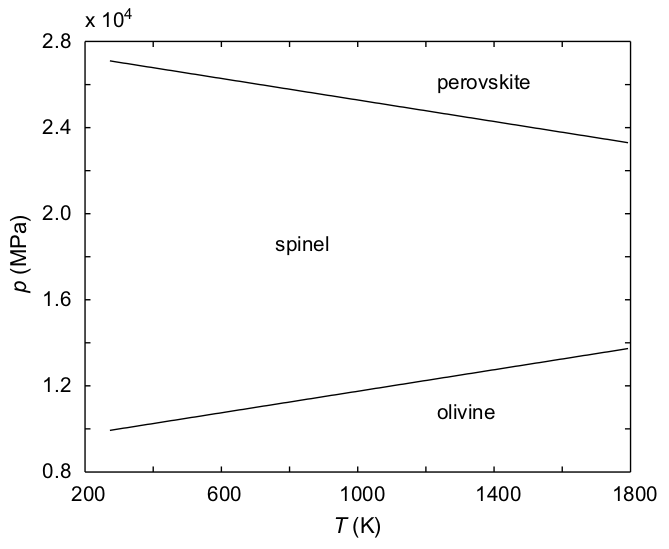
\includegraphics[width=7cm]{images/phasetransitions/zldf07}\\
{\captionfont Phase diagram indicating stable mineral phases in the 
temperature-pressure plane. The phase diagram is divided into three regions
corresponding to three distinct minerals: olivine, spinel and perovskite.
Taken from \cite{zldf07}.}
\end{center}

They state that two major mineralogical phase transitions occur, one at
410 km depth and other at 660 km depth (other deeper transitions run outside the 
domain under study because their domain is 1000km deep). The density increases 
discontinuously across these phase transitions. 
In order to take into account the effect of these 
discontinuities, the density $\rho_0$ above is taken as a reference density plus an 
increment $\Delta \rho$:
\[
\rho_0 = \rho_{olivine} + \Delta \rho
\]
where 
\[
\Delta \rho
=
\left\{
\begin{array}{lll}
0 & \text{if } (T,p) \text{is in the olivine region} \\
\Delta \rho_{es} & \text{if } (T,p) \text{is in the spinel region} \\
\Delta \rho_{per} & \text{if } (T,p) \text{is in the perovskite region} 
\end{array}
\right.
\]
The authors unfortunately fail to report how the phase transitions affect the viscosity.

The obvious problem with this otherwise simple approach is that density varies in the domain but 
is not accompanied by a volume change so that it violates mass conservation.

\item the following phase diagram is taken from Peltier et al (1997) \cite{pebs97}.

\begin{center}
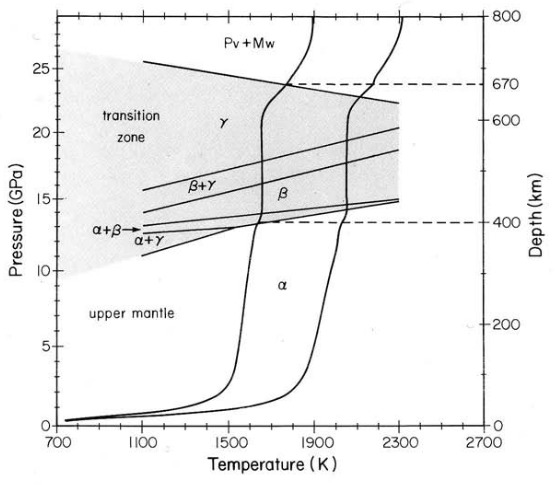
\includegraphics[width=7cm]{images/phasetransitions/pebs97}\\
{\captionfont Phase boundary for the $\alpha \rightarrow \beta \rightarrow \gamma$ transitions of 
Olivine}
\end{center}


\end{itemize}


\begin{center}
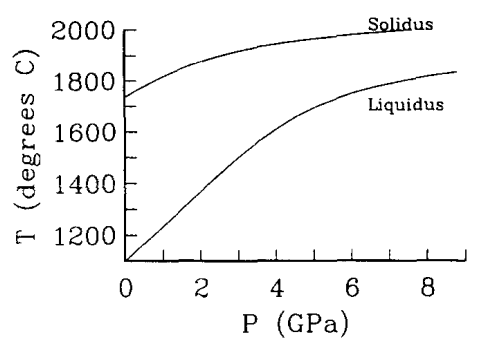
\includegraphics[width=6cm]{images/phasetransitions/kian95a}
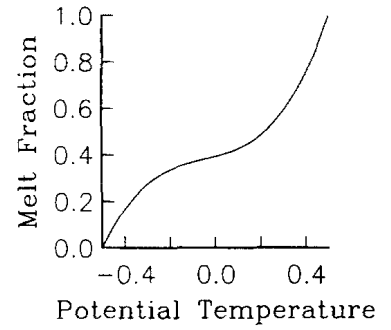
\includegraphics[width=5cm]{images/phasetransitions/kian95b}\\
{\captionfont Left: Solidus and liquidus temperatures; 
Right: melt fraction as a function temperature for dry peridotite.
Taken from King \& Anderson (1995) \cite{kian95}, 
Both after McKenzie \& Bickle \cite{mcbi88}.}
\end{center}

\begin{center}
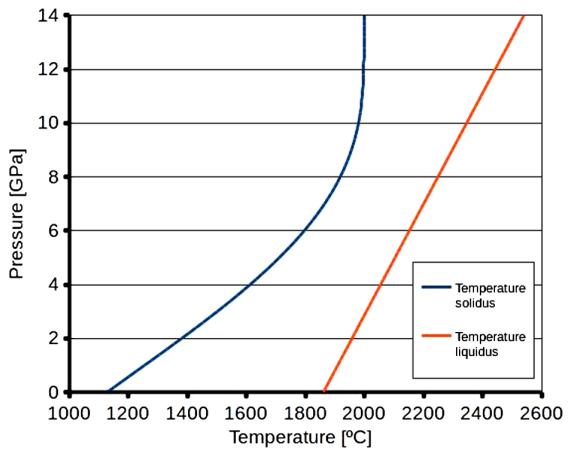
\includegraphics[width=6cm]{images/phasetransitions/latb17}\\
{\captionfont Left: Solidus and liquidus curves. 
Taken from Lavecchia et al (2017) \cite{latb17}.} 
\end{center}




\Literature: \cite{scyt75}
